% ---------------------------------------------------------------------------------------
%  FIGURE 4.4 — state coverage.  Drop this wherever the mechanism is first argued.
%  ASSET: figures/fig_state_coverage.pdf
%    Regenerate:  PYTHONPATH=. python -m experiments.make_fig_state_coverage
%
%  READ THE CAPTION CAREFULLY BEFORE EDITING IT. The matched-sample-size qualifier is not
%  hedging -- without it the result reverses to a near-tie (37.7% vs 32.8%), because planner
%  episodes run to horizon 900 against 300 and contribute ~30x more state points per scene.
%  Any rewording that drops "at matched sampling" makes the figure indefensible.
% ---------------------------------------------------------------------------------------

\begin{figure}[htbp]
  \centering
  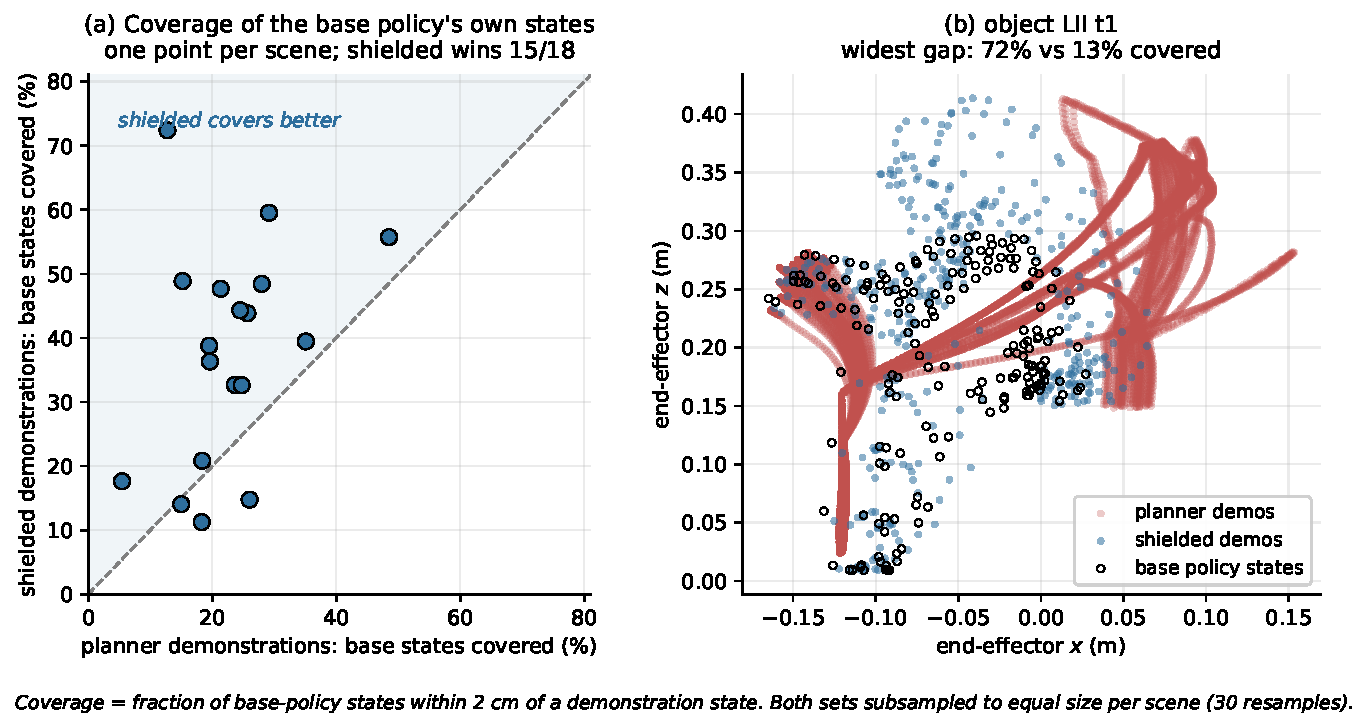
\includegraphics[width=\linewidth]{figures/fig_state_coverage.pdf}
  \caption[State coverage of the base policy's own trajectories]{%
    The mechanism, measured. Coverage is the fraction of the base policy's visited
    end-effector states lying within 2\,cm of some demonstration state, with both
    demonstration sets subsampled to equal size per scene (30 resamples) so that the
    comparison is not confounded by the planner's longer episodes.
    \textbf{(a)} One point per scene: the shielded rollouts cover the policy's own states
    better in 15 of 18 scenes, 37.7\% against 22.8\% pooled.
    \textbf{(b)} The same comparison on the widest-gap scene. The planner's demonstrations
    form tight, near-deterministic trajectory bands, while the states the policy actually
    visits are diffuse and largely elsewhere.
    Coverage is computed on end-effector position only --- three of the eight observed
    dimensions, and not joint configuration --- so it supports the state-coverage account
    without exhausting it.}
  \label{fig:state_coverage}
\end{figure}
